\begin{frame}{Work-stealing}
\centering
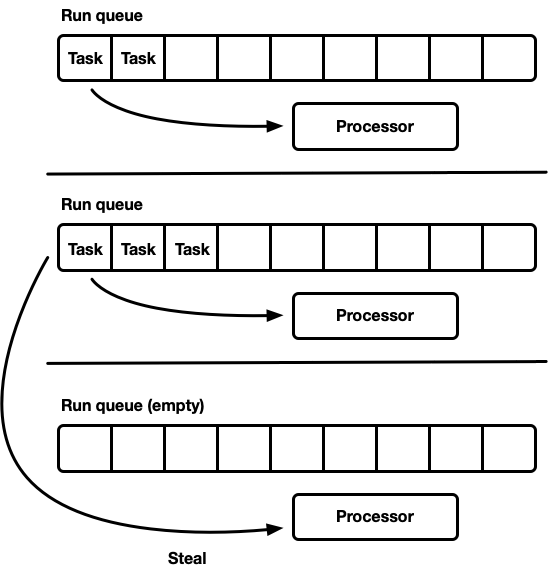
\includegraphics[scale=0.37]{images/work_stealing.png}
\end{frame}

% ---------------------------------------------------------

\begin{frame}{Work-stealing algorithms}
\begin{enumerate}
	\item Frigo, Leiserson \& Randall (1998)
		\begin{itemize}
			\item at the core of Cilk~5
			\item lock
		\end{itemize}
	\item Arora, Blumofe \& Plaxton (2001)
		\begin{itemize}
			\item no lock
			\item one fixed size array (not circular), can overflow
		\end{itemize}
	\item Hendler, Lev \& Shavit (2004)
		\begin{itemize}
			\item no lock
			\item list of small size arrays, no overflow
		\end{itemize}
	\item \underline{Chase \& Lev (2005)}
		\begin{itemize}
			\item no lock
			\item circular arrays, no overflow
		\end{itemize}
\end{enumerate}
\end{frame}